\documentclass[a4paper,12pt]{article}
\usepackage[utf8]{inputenc}
\usepackage[T1]{fontenc}
\usepackage[spanish]{babel}
\spanishdecimal{.}
\usepackage{csquotes}
\usepackage{anysize}
\usepackage{graphicx}
\usepackage[colorlinks=true]{hyperref}
\usepackage{subcaption}
\marginsize{25mm}{25mm}{25mm}{25mm}
\linespread{1.5}

\title{Tasa de defunción y recuperación de {\scshape Covid-19} durante la primera mitad de 2020 en México}
\author{Daniel Maldonado}
\date{\today}

\begin{document}
{\bfseries \maketitle}

Se obtuvo una base de datos relacionada con la incidencia de COVID-19 a nivel nacional durante la primera mitad del año 2020.
La base de datos se encuentra disponible haciendo clic \href{https://datos.cdmx.gob.mx/dataset/casos-asociados-a-covid-19/resource/1943a45c-542b-4ac2-a319-cd8da9ba36f1}{aquí}.

La base de datos contiene información de casos referentes a personas que acudieron a una Unidad Médica de gobierno debido a sospecha de COVID-19.
La base contiene información de casos confirmados positivos, sospechosos, y negativos, por lo que es necesario filtrar antes de hacer un análisis más profundo.
De igual forma, la base no contiene una columna que indique de forma explícita si un caso resultó en una defunción o recuperación: esto debe computarse con base en la presencia de una fecha de defunción.

Se realizó un análisis en dos partes de manera paralela con el propósito de corroborar los resultados: un reporte en Power BI y un análisis con la librería Pandas de Python.
Ambos análisis entregaron resultados consistentes, lo que da validez a ambos métodos.

Se descubrió que el total de defunciones debidas a casos confirmados de {\scshape Covid-19} durante la primera mitad de 2020 fue de 11,503.
Mientras, 62,481 casos confirmados como positivos terminaron en una recuperación.
No se analizaron los casos negativos, sospechosos, o con poca evidencia de laboratorio.

Una segmentación por sexo (figura \ref{fig:def_rec_por_sexo}) mostró que, de las 11,503 defunciones, 7,836 fueron de hombres y 3,667 fueron de mujeres.
Por otro lado, de las 62,481 recuperaciones 32,454 fueron de hombres y 30,027 fueron de mujeres.
Es decir, {\slshape {\bfseries aunque hombres y mujeres se recuperaron en proporciones similares, los hombres tenían más del doble de probabilidad de morir}}.

\begin{figure}[!ht]
    \begin{center}
	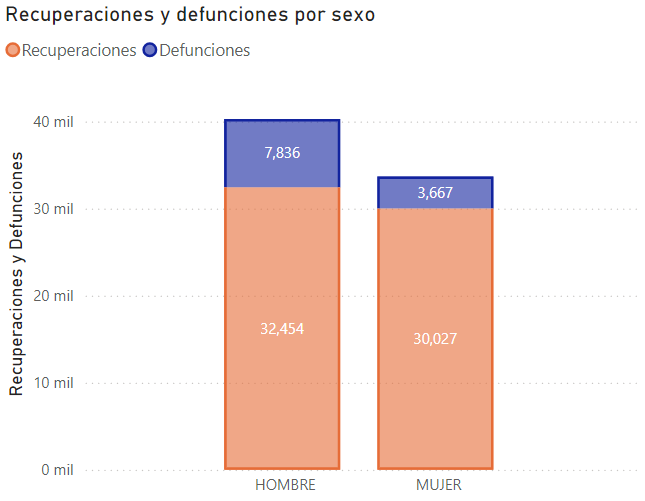
\includegraphics[scale=0.6]{Def_rec_por_sexo.png}
    \end{center}
    \captionsetup{width=\linewidth}
    \caption{Defunciones y recuperaciones por sexo.}
    \label{fig:def_rec_por_sexo}
\end{figure}

Un análisis de serie de tiempo (figura \ref{fig:def_por_tiempo}) reveló la tendencia ya conocida de los casos de {\scshape Covid-19}: una ola con un pico alrededor del 15 de Mayo y una caída poco tiempo después.

\begin{figure}[!ht]
    \begin{center}
	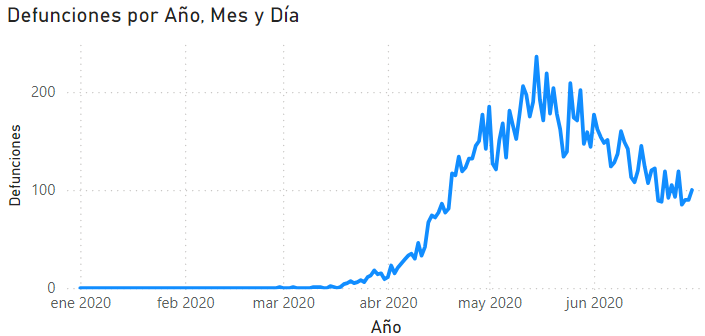
\includegraphics[scale=0.6]{Def_por_tiempo_powerbi.png}
    \end{center}
    \captionsetup{width=\linewidth}
    \caption{Defunciones en función del tiempo.}
    \label{fig:def_por_tiempo}
\end{figure}

Un análisis posterior, igualmente de serie de tiempo (figura \ref{fig:def_rec_por_tiempo}) mostró que las recuperaciones siguieron la misma tendencia, pero con valores mucho mayores.

Este análisis mostró un patrón interesante en los datos de recuperaciones: se presentan conteos anormalmente bajos a intervalos regulares, representados como picos hacia abajo en la gráfica.
Estos picos son formados por dos días separados por cinco días de actividad normal.
{\slshape {\bfseries Comparar este patrón con las fechas de calendario correspondientes reveló que cada pico coincide con días sábado y domingo, es decir, que probablemente se trata de un error de captura relacionado con la poca actividad durante los fines de semana.}}

\begin{figure}[!ht]
    \begin{center}
	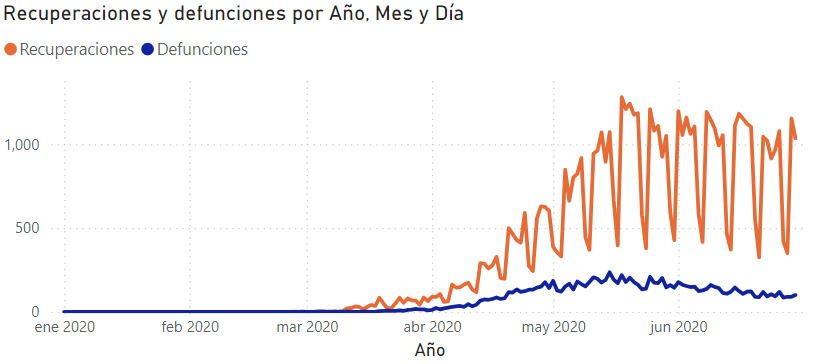
\includegraphics[scale=0.6]{Def_rec_por_tiempo.png}
    \end{center}
    \captionsetup{width=\linewidth}
    \caption{Defunciones y recuperaciones en función del tiempo.}
    \label{fig:def_rec_por_tiempo}
\end{figure}

Por otro lado, una segmentación por entidad federativa mostró que la mayor parte tanto de defunciones como de recuperaciones fueron registradas en la Ciudad de México; mientras, una proporción menor fue registrada en el Estado de México, y una porción muy pequeña en el resto del país (figura \ref{fig:def_por_entidad}).

\begin{figure}[!ht]
    \begin{center}
	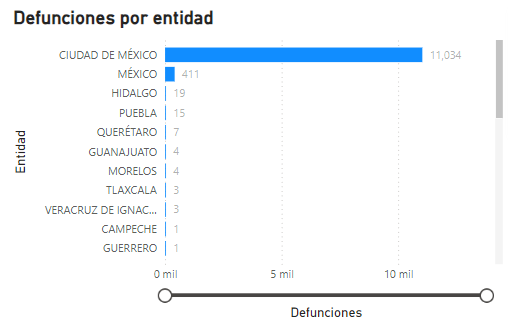
\includegraphics[scale=0.8]{Def_por_entidad_powerbi.png}
    \end{center}
    \captionsetup{width=\linewidth}
    \caption{Total de defunciones por entidad federativa.}
    \label{fig:def_por_entidad}
\end{figure}

Finalmente, un análisis de la tasa de defunción y recuperación en función de la edad (figura \ref{fig:def_rec_por_edad}) sugiere que {\bfseries {\slshape la población con la mayor probabilidad de morir dado un diagnóstico positivo de {\scshape Covid-19} es la de tercera edad; mientras, la población con la mayor probabilidad de recuperarse es la población joven, por debajo de los 50 años.}}

\begin{figure}[!ht]
    \begin{center}
	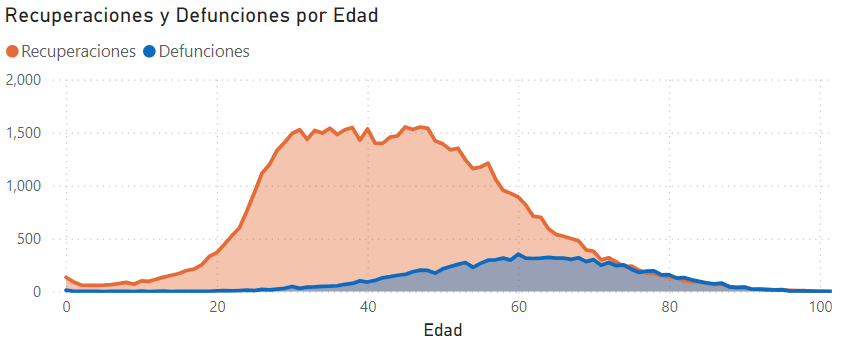
\includegraphics[scale=0.6]{Def_rec_por_edad.png}
    \end{center}
    \captionsetup{width=\linewidth}
    \caption{Defunciones y recuperaciones por edad.}
    \label{fig:def_rec_por_edad}
\end{figure}


\end{document}
